\documentclass[notheorems,mathserif,table,compress]{beamer}  %dvipdfm选项是关键,否则编译统统通不过
%%------------------------常用宏包------------------------
%%注意, beamer 会默认使用下列宏包: amsthm, graphicx, hyperref, color, xcolor, 等等
\usepackage{fontspec,xunicode,xltxtra}  % for XeTeX
\usepackage{verbatim}
\usepackage{mathabx}
\usepackage{tcolorbox}
\usepackage{subfigure} %%图形或表格并排排列
\usepackage{colortbl,dcolumn}     %% 彩色表格
\usepackage{styles/zhfontcfg}
\usepackage{styles/iplouclistings}
\usepackage{listings}
\usepackage{styles/iplouccfg}
\usepackage{fancybox}     %% 定义zhushadow时用到
\usepackage{verbatim}
\newsavebox{\mysaveboxOne}  %%为了在only中使用lstlisting
\newsavebox{\mysaveboxTwo}
\newsavebox{\mysaveboxThree}
\newsavebox{\mysaveboxFour}
\newsavebox{\mysaveboxFive}
\newsavebox{\mysaveboxSix}
%%------------------------ThemeColorFont------------------------
\usetheme{Madrid}
\usecolortheme{whale}      % Outer color themes, 其他选择: whale, seahorse, dolphin . 换一个编译看看有什么不同.
\usecolortheme{orchid}     % Inner color themes, 其他选择: lily, orchid
\useinnertheme[shadow]{rounded}
\useoutertheme{miniframes} 
\usefonttheme{serif}
\setbeamertemplate{background canvas}[vertical shading][bottom=white,top=structure.fg!7] %%背景色, 上25%的蓝, 过渡到下白.
\setbeamertemplate{theorems}[numbered]
\setbeamertemplate{navigation symbols}{}   %% 去掉页面下方默认的导航条.

\newcommand\zhushadow[2][purple]{\hskip5pt\shadowbox{\color{#1}\small\kai #2\vspace{3mm}}}

%%------------------------LOGO------------------------
\pgfdeclareimage[height=1cm]{university-logo}{Git-Logo-2Color.png}
\logo{\pgfuseimage{university-logo}}
%%----------------------------------------------------

%%------------------------MISC------------------------
\graphicspath{{figures/}}         %% 图片路径. 本文的图片都放在这个文件夹里了.
%%------------------------正文------------------------
\begin{document}
\XeTeXlinebreaklocale "zh"         % 表示用中文的断行
\XeTeXlinebreakskip = 0pt plus 1pt % 多一点调整的空间
%%----------------------------------------------------------
%% This is only inserted into the PDF information catalog. Can be left
%% out.
%%%
%% Delete this, if you do not want the table of contents to pop up at
%% the beginning of each subsection:
\AtBeginSection[]{                              % 在每个Section前都会加入的Frame
  \frame<handout:0>{
    \frametitle{Agenda}\small
    \tableofcontents[current,currentsubsection]
  }
}

\AtBeginSubsection[]                            % 在每个子段落之前
{
  \frame<handout:0>                             % handout:0 表示只在手稿中出现
  {
    \frametitle{Agenda}\small
    \tableofcontents[current,currentsubsection] % 显示在目录中加亮的当前章节
  }
}

%%----------------------------------------------------------
\title{开源软件之——git学习篇}
\author[zhu]{主讲人~~~~~\textcolor{olive}{朱亚菲}\\
    \quad 幻灯片制作~~\textcolor{olive}{赵海伟、朱亚菲}}
\institute[CVBIOUC]{\small\textcolor{violet}{CVBIOUC\\
\url{http://vision.ouc.edu.cn/~zhenghaiyong}}}
\date{2014~年~9~月~19~日} 
%\titlegraphic{\vspace{-6em}\includegraphics[height=7cm]{ouc}\vspace{-6em}}
\frame{ \titlepage }
%%----------------------------------------------------------

\frame{\frametitle{Contents}\tableofcontents}

%%----------------------------------------------------------
\section{Git简介}

\subsection{Git是什么?}

\begin{frame}
  \zhushadow{Git} Git是目前世界上最先进的分布式版本控制系统!

\pause

  \zhushadow{版本控制} 

  \begin{columns}
  \begin{column}{0.3\textwidth} 
  \includegraphics[width=\linewidth]{word.png}
  \end{column}
  \hspace{-7em}
  \begin{column}{0.1\textwidth} 
  \begin{flushleft}
  \centering\rowcolors[]{1}{blue!20}{blue!10}
  \resizebox{3\hsize}{!}{$\begin{tabular}{|c|c|c|c|c|}  
  \hline
  版本 & 用户  &        说明            &    日期       \\
  \hline
    1  & 张三  & 删除了实验室规则说明5   & 7/12 10:38   \\ 
  \hline
    2  & 李四  &     加入一幅图片       &  7/12 18:09   \\
  \hline
    3  & 张三  &   修改了README.md      &  7/13 9:51    \\
  \hline
    4  & 李四  &   新增一种绘图颜色      &  7/14 15:17   \\
  \hline 
  \end{tabular}$}
  \end{flushleft}
  \vspace{2em}
  \end{column}
  \end{columns}

\pause

  \zhushadow{集中式vs分布式} 
  \begin{figure}
  \vspace{-1mm}
  \begin{minipage}[t]{0.2\linewidth} 
    \centering 
    \includegraphics[width=\linewidth]{集中式.png} \\
    {\heiti\textcolor{blue}{集中式}}
  \end{minipage}
  \hspace{2cm}
  \begin{minipage}[t]{0.2\linewidth}
    \centering 
    \includegraphics[width=\linewidth]{分布式.png} \\
    {\heiti\textcolor{blue}{分布式}}
  \end{minipage}
\end{figure}
\end{frame}


\subsection{Git的诞生}

\begin{frame}
  \begin{itemize}
  \item 1991-2002年间,世界各地的志愿者把源代码文件通过diff的方式发给Linus,然后由Linus本人通过手工方式合并代码!
  \item 到2002年,整个项目组开始启用分布式版本控制系统BitKeeper来管理和维护代码。
  \item 到了2005年,开发BitKeeper的商业公司同Linux内核开源社区的合作关系结束,他们收回了免费使用BitKeeper的权力。这就迫使 Linux开源社区不得不吸取教训,只有开发一套属于自己的版本控制系统才不至于重蹈覆辙。
  \item Linus花了两周时间自己用C写了一个分布式版本控制系统,这就是Git!一个月之内,Linux系统的源码已经由Git管理了!
  \end{itemize}
\end{frame}

\section{Git使用}

\subsection{基础}

\begin{frame}[fragile]
  \frametitle{使用Git前的准备工作}
  \begin{enumerate}
  \item 安装
  \item 设置

  \verb|$git config --global user.name "Your Name"|\\
  \verb|$git config --global user.email "email@example.com"|
  \item 创建版本库

  \hspace{0.2em}\vspace{1em}\includegraphics[width=7cm]{repository.png}
  \end{enumerate}
\end{frame}


%\begin{frame}[fragile]
%  \begin{lstlisting}
%  $git config --global user.name "Your Name"
%  $git config --global user.email "email@example.com"
%  \end{lstlisting}
%  \verb|$git config --global user.name "Your Name"|
%  \\
%  \verb|$git config --global user.email "email@example.com"|
%\end{frame}

%\begin{frame}[fragile]
%\frametitle{}
%\only<1>{
%\begin{center}
%\fbox{\$git log --pretty=oneline FileName}
%\\
%\includegraphics[width=5cm]{log.png}
%\end{center}
%}
%\only<2>{
%\begin{center}
%\fbox{\$git show aa31c}
%\\
%\includegraphics[width=5cm]{gitshow.png}
%\end{center}
%}
%\end{frame}

%\begin{frame}[fragile]
%\frametitle{}
%\begin{columns}
%\column{0.6\textwidth}
%\verb|$git log --pretty=oneline FileName|
%\\
%\includegraphics[width=5cm]{log.png}
%\column{0.4\textwidth}
%\verb|$git show aa31c|
%\\
%\includegraphics[width=5cm]{gitshow.png}
%\end{columns}
%\end{frame}


\begin{frame}
  \frametitle{记录每次更新到仓库}
  \centering\includegraphics[width=10cm]{FileStatus.png}
\end{frame}


\begin{frame}
  \frametitle{查看某个文件的修改历史}
  \begin{tcolorbox}[colback=blue!5,colframe=blue!75!black] 
  \begin{columns}
  \begin{column}{0.5\textwidth}
  \begin{center}
  \begin{tabular}{|l|}
  \hline
  \$git log $-$$-$pretty=oneline 文件名\\
  \hline
  \end{tabular}
  \includegraphics[width=5cm]{log.png}
  \end{center}
  \end{column}

  \begin{column}{0.5\textwidth}
  \begin{center}
  \begin{tabular}{|l|}
  \hline
  \$git show aa31c\\
  \hline
  \end{tabular}
  \includegraphics[width=5cm]{gitshow.png}
  \end{center}
  \end{column}
  \end{columns}
  \end{tcolorbox}
\end{frame}


\begin{frame}
  \frametitle{Git的杀手级功能之一:远程仓库}
  \zhushadow{服务器} 找一台电脑充当服务器的角色,每天24小时开机,其他每个人都从这个“服务器”仓库克隆一份到自己的电脑上,并且各自把各自的提交推送到服务器仓库里,也从服务器仓库中拉取别人的提交。
  \zhushadow{Github} Github是一个共享虚拟主机服务,用于存放使用Git版本控制的软件代码和内容项目。
\end{frame}

\subsection{分支管理}

\begin{frame}
  \frametitle{Git的杀手级功能之二:分支模型}
  \zhushadow{分支} 每次提交,Git都把它们串成一条时间线,这条时间线就是一个分支。

  \zhushadow{应用场景} 假设你准备开发一个新功能,但是需要两周才能完成,如果代码还没写完就提交,不完整的代码库会导致别人无法工作,如果等代码全部写完再一次提交,又存在丢失每天进度的巨大风险。
\end{frame}


\begin{frame}[fragile]
  \frametitle{HEAD}
  \begin{itemize}
  \item HEAD文件是一个指向你当前所在分支的引用标识符。
  \begin{lstlisting}
  $cat .git/HEAD 
  ref: refs/heads/master
  \end{lstlisting}
  \item 如果你执行git checkout dev, Git就会更新这个文件:
  \begin{lstlisting}
  $cat .git/HEAD 
  ref: refs/heads/dev
  \end{lstlisting}
  \end{itemize}
\end{frame}

  \begin{lrbox}{\mysaveboxOne}
  \verb|$git branch|
  \end{lrbox}

  \begin{lrbox}{\mysaveboxTwo}
  \verb|$git checkout -b dev|
  \end{lrbox}
  
  \begin{lrbox}{\mysaveboxThree}
  \verb|$git checkout master|
  \end{lrbox}

  \begin{lrbox}{\mysaveboxFour}
  \verb|$git merge dev|
  \end{lrbox}

  \begin{lrbox}{\mysaveboxFive}
  \verb|$git branch -d dev|
  \end{lrbox}

\begin{frame}[fragile]
  \frametitle{创建与合并分支}
  \only<1>{
  \begin{center}
  
\includegraphics[width=0.5\linewidth]{1.png}
  \newline
  \usebox{\mysaveboxOne}
  \end{center}}

  \only<2>{
  \begin{center}
  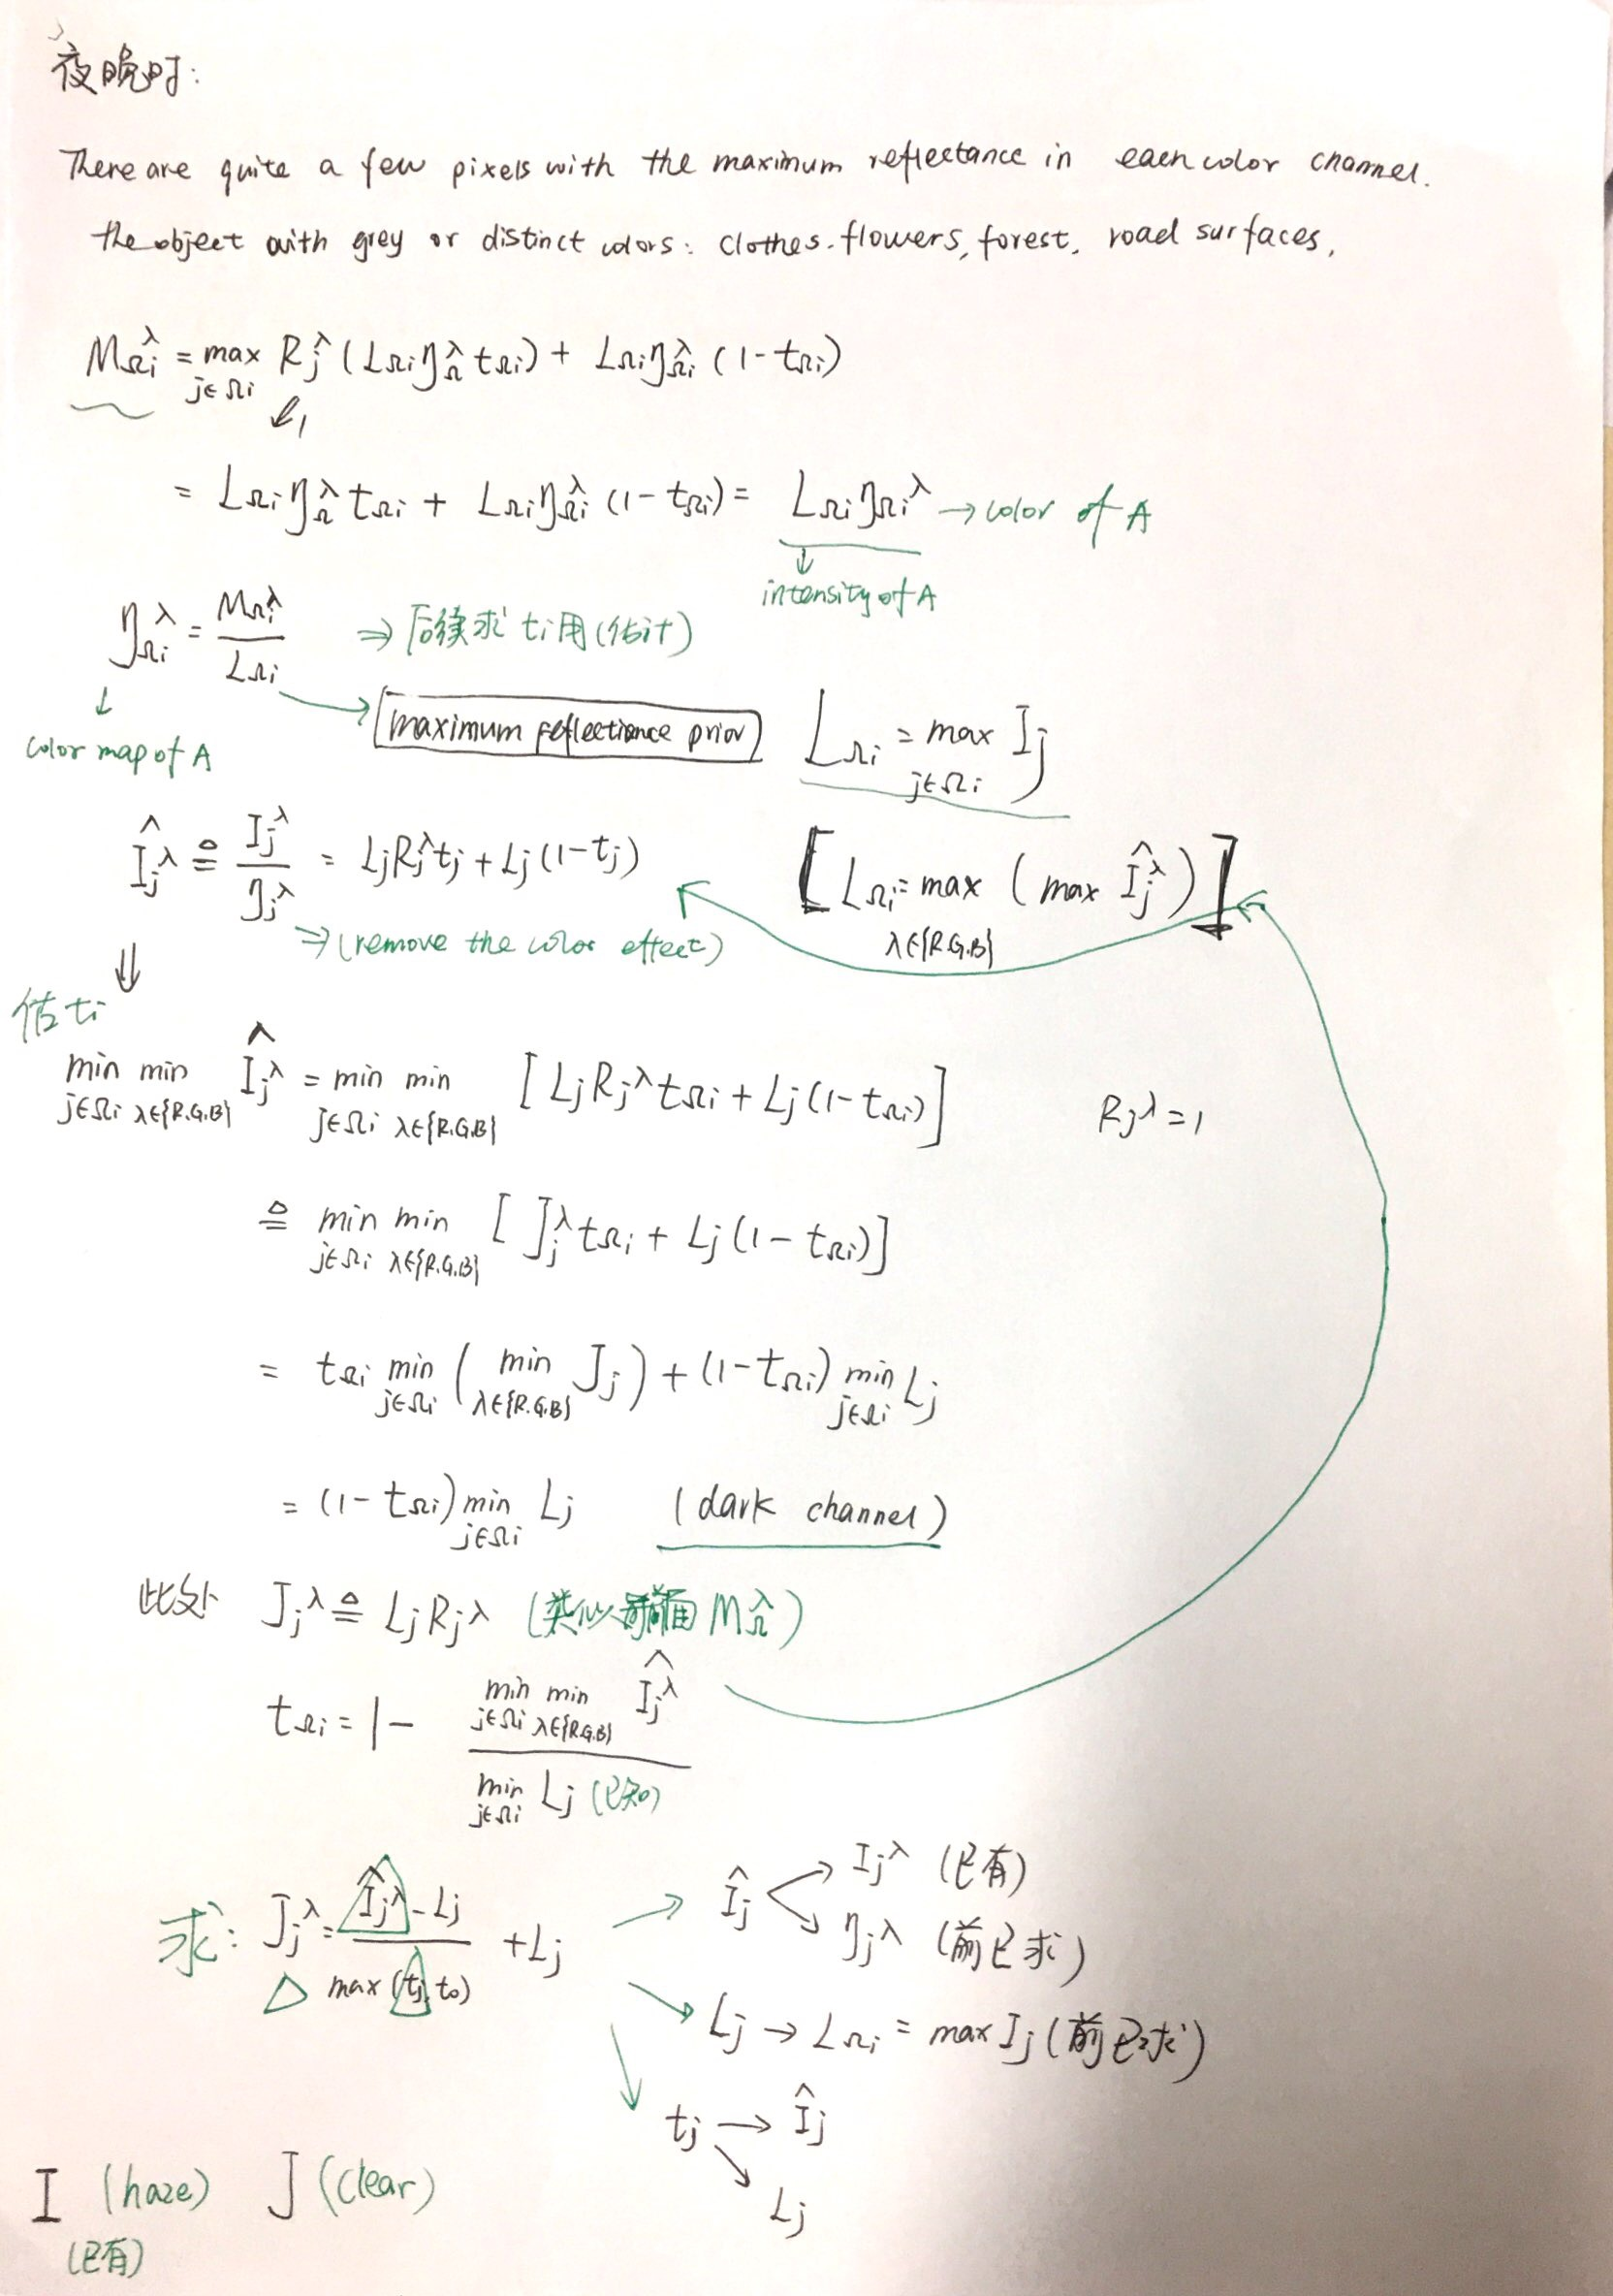
\includegraphics[width=0.5\linewidth]{2.png}
  \newline
  \usebox{\mysaveboxTwo}
  \end{center}}

  \only<3>{
  \begin{center}
  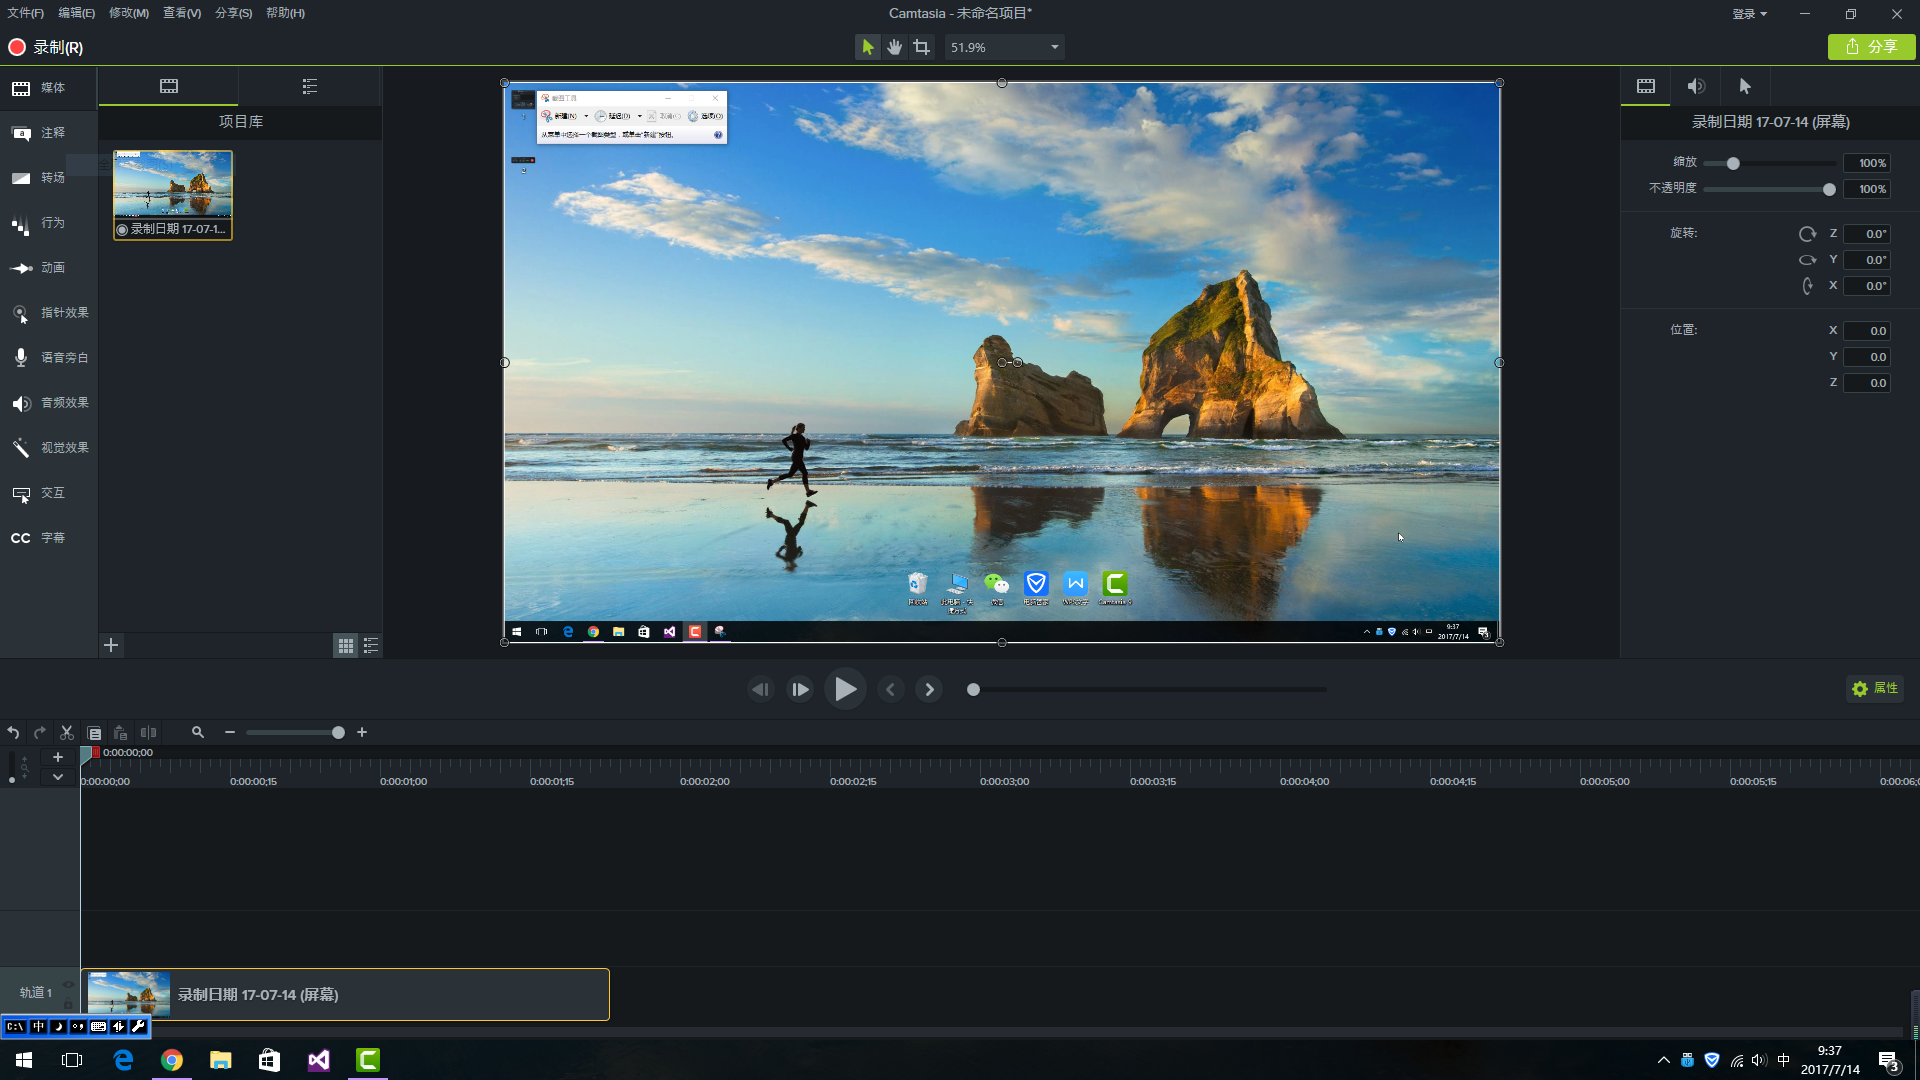
\includegraphics[width=0.5\linewidth]{3.png}
  \end{center}}

  \only<4>{
  \begin{center}
  
\includegraphics[width=0.5\linewidth]{4.png}
  \newline
  \usebox{\mysaveboxThree}
  \newline
  \usebox{\mysaveboxFour}
  \end{center}}

  \only<5>{
  \begin{center}
  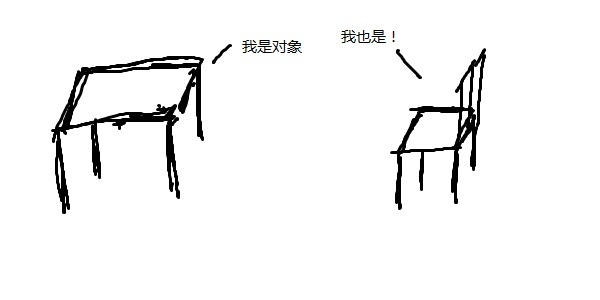
\includegraphics[width=0.3\linewidth]{5.png}
  
\includegraphics[width=0.3\linewidth]{1.png}
  \newline
  \usebox{\mysaveboxFive}
  \end{center}}
\end{frame}


\begin{frame}
  \frametitle{分支管理策略}
  \begin{itemize}
  \item master分支应该是非常稳定的,也就是仅用来发布新版本,平时不能在上面工作。
  \item dev分支是不稳定的,平时在dev分支上工作,到某个时候,比如1.0版本发布时,再把dev分支合并到master上,在master分支发布1.0版本。
  \item 团队中的每个人都在dev分支上干活,每个人都有自己的分支,时不时地往dev分支上合并。
  \end{itemize}
\end{frame}


\begin{frame}
  \frametitle{储藏现场}
  \zhushadow{应用场景} 当你接到修复代号100的bug的任务时,很自然地,你想创建一个分支issue-100来修复它,但是当前正在dev分支上进行的工作还没有提交,并不是你不想提交,而是工作只进行到一半,还没法提交,预计完成还需1天时间,但是必须在两个小时内修复该bug。
  
  \begin{itemize}
  \item 使用git stash命令把当前工作现场“储藏”起来,等以后恢复现场后继续工作。
  
  \end{itemize}
\end{frame}

\section{Github与CVBIOUC}

\begin{frame}
  \frametitle{实验室中的使用场景}
  实验室Github网址: \url{https://github.com/zhenglab}

  \begin{itemize}
  \item 写论文
  \item 代码管理
  \item 每周汇报记录
  \item 软件使用说明
  \item $\cdots$
  \end{itemize}
\end{frame}


\begin{frame}
  \frametitle{My Project}
  \centering\includegraphics[width=10cm]{saliency.png}
\end{frame}


\begin{frame}
  \frametitle{README}
  \centering\includegraphics[width=10cm]{readme.png}
\end{frame}


\begin{frame}
  \frametitle{实验室每周例会记录}
  \centering\includegraphics[width=10cm]{WeeklyMeetings.png}
\end{frame}


\begin{frame}
  \frametitle{说明文档}
  \centering\includegraphics[width=9cm]{Git-Github-howto.png}
\end{frame}


\begin{frame}
  \vspace{2cm}
  \centering
  \zhushadow{\color{blue}\Huge{Thanks}}\\
  \vspace{1.5cm}
  \begin{flushright}
  \emph{\href{mailto:bingzh@ouc.edu.cn}{Yafei~Zhu}}\\
  \href{http://www.ouc.edu.cn}{Ocean University of China}\\
  \emph{2014.09}
  \end{flushright}  
\end{frame}
\end{document}
